\newpage
\section{Anonymisering av bilder med ansikter}
\label{sec:Anonymisering}
\subsection{Bakgrunn}
Anonymisering av bilder er enkelte ganger nødvendig før det blir offentlig vist frem for å skjerme den avbildedes personvern. En teknikk som ofte blir brukt er å gjøre ansiktene uskarpe og resten av bildet forblir skarpt. Teknikken avhenger av at programmet klarer å gjenkjenne ansiktene\cite{wiki:FaceDetection} for å definere en maske rundt, slik at man kan isolere anvendingen av bildet kun på ansiktet, og i likhet som tidligere er det flere teknikker som benyttes. I denne oppgaven brukte vi biblioteket OpenCV (Open Source Computer Vision Library) og maskinlæringsalgoritmen Haar Cascade. 



\subsubsection{Open CV}
Open CV er et open source datasyn-\cite{datasyn} og maskinlæringsbibliotek som ble utviklet for å skape et felles infrastruktur for datasynsapplikasjoner og for å akselerere bruken av maskinoppfatning i kommersielle produkter\cite{cv2}. Kort fortalt betyr dette datamaskinens evne til å tolke data på en måte som ligner på hvirdan mennesker bruker sansene til å oppfatte verden rundt seg\cite{wiki:machinePerception}, og da spesielt synet i dette tilfellet.  

\subsubsection{Haar Cascade algoritmen}
Haar Cascade er en maskinlæringsalgoritme~\cite{haar} som brukes til å identifisere objekter i et bilde eller i en video. Den er mest kjent til å identifisere ansikter, men kan trenes til å identifisere nesten hva det måtte være av objekter.

Algoritmen trenger å trenes med flere positive bilder av ansikter og negative bilder uten ansikter, deretter må man trekke ut kjente egenskaper fra disse bildene. Første steget er å samle inn Haar-features. 

De to første elementene (figur \ref{fig:haarfeat}) kalles for edge-features som benyttes til å detektere kanter i objekter. Den tredje er en line-feature, mens den fjerde heter four rectangle-feature som oftest benyttes til å gjengkjenne en skrå linje.

Haar-Features er veldig god til å gjenkjenne linjer og kanter på objekter, og spesielt i ansikter. Som man ser i (figur \ref{fig:haarface}) klarer en edge-feature å gjengkjenne essensielle deler ved et ansikt, som f.eks et øye. Grunnen til dette er at i bildet blir det en kontrast mellom øyet og kinnet, som kan minne om objekt 2 fra figur (\ref{fig:haarfeat}), altså en mørk overdel med lys bunn.

\begin{figure}
\begin{center}
    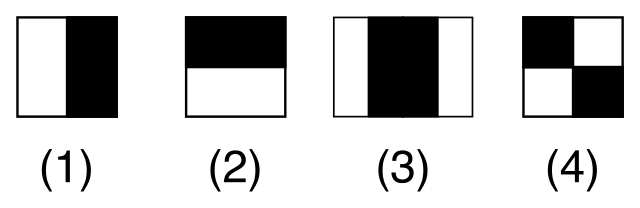
\includegraphics[width=0.4\columnwidth]{bilder/Anonymisering/VJ_featureTypes.svg.png}
     \caption{Haar Feature\label{fig:haarfeat}} \source{Wikimedia Commons~\cite{wiki:haarfeat}}
\end{center}
\end{figure}

\begin{figure}
\begin{center}
    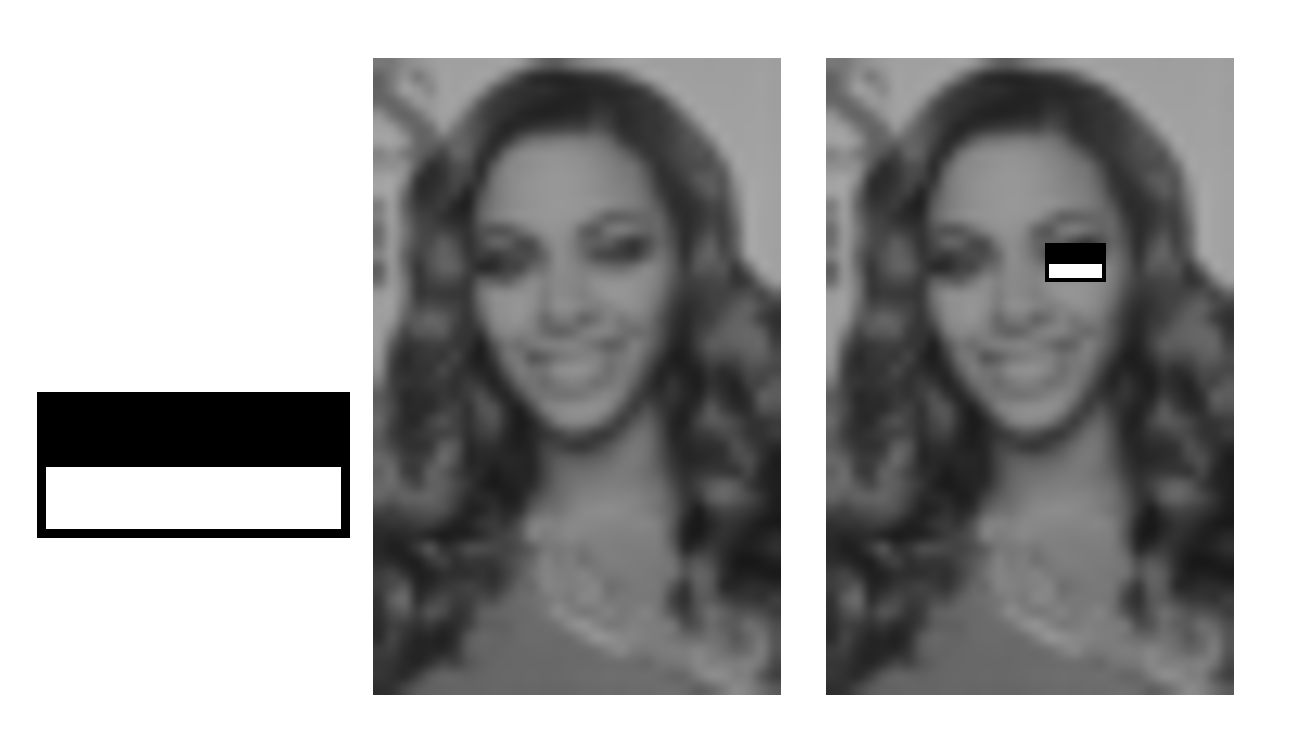
\includegraphics[width=0.5\columnwidth]{bilder/Anonymisering/haarface-example.png}
     \caption{Haar Feature demonstrert på et ansikt \label{fig:haarface}} \source{Wikimedia Commons~\cite{wiki:haarface}}
\end{center}
\end{figure}
 
%\import{./kode/}{anonymiseringModul}
%\begin{center}
%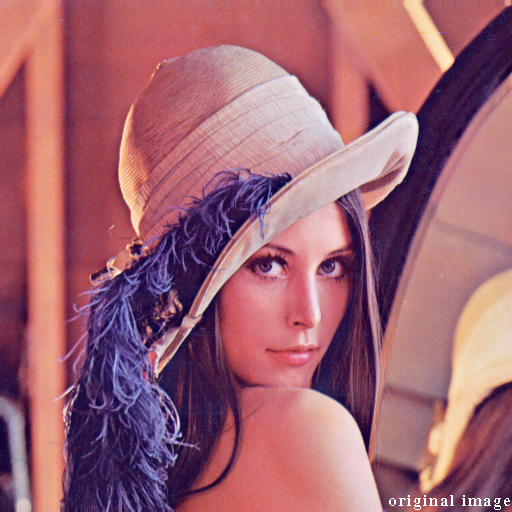
\includegraphics[scale = 0.3]{./bilder/Anonyme/lena.png}
%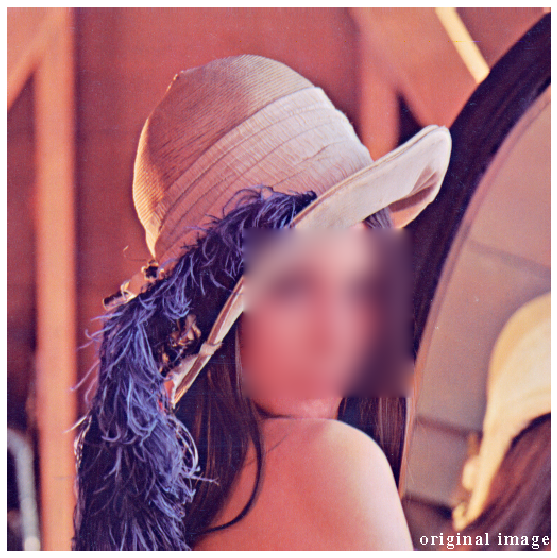
\includegraphics[scale = 0.28]{./bilder/Anonyme/lenaBlur.png}
%\end{center}